
\begin{figure}[!tp]
     \centering
     \begin{subfigure}[b]{0.49\textwidth}
         \centering
         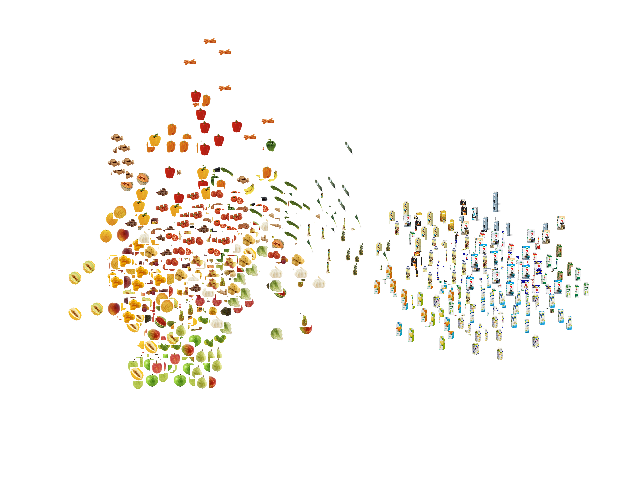
\includegraphics[width=\textwidth]{PaperB/figures_and_tables/latent_space_visualizations/pca_latents_vcca_xw_seed2.png}
         \caption{$\mu_{z}$ from VCCA$_{x w}$}
         \label{fig:pca_vcca_xw_z}
     \end{subfigure} 
     \begin{subfigure}[b]{0.49\textwidth}
         \centering
         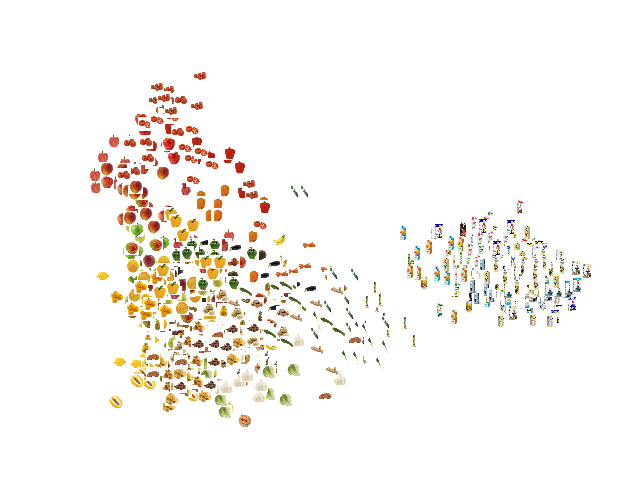
\includegraphics[width=\textwidth]{PaperB/figures_and_tables/private_latent_space_visualizations/pca_z_vaecca_private_xw_seed1.png}
         \caption{$\mu_{z}$ from VCCA-private$_{x w}$}
         \label{fig:pca_vcca_private_xw_z}
     \end{subfigure} \\
     \begin{subfigure}[b]{0.6\textwidth}
         \centering
         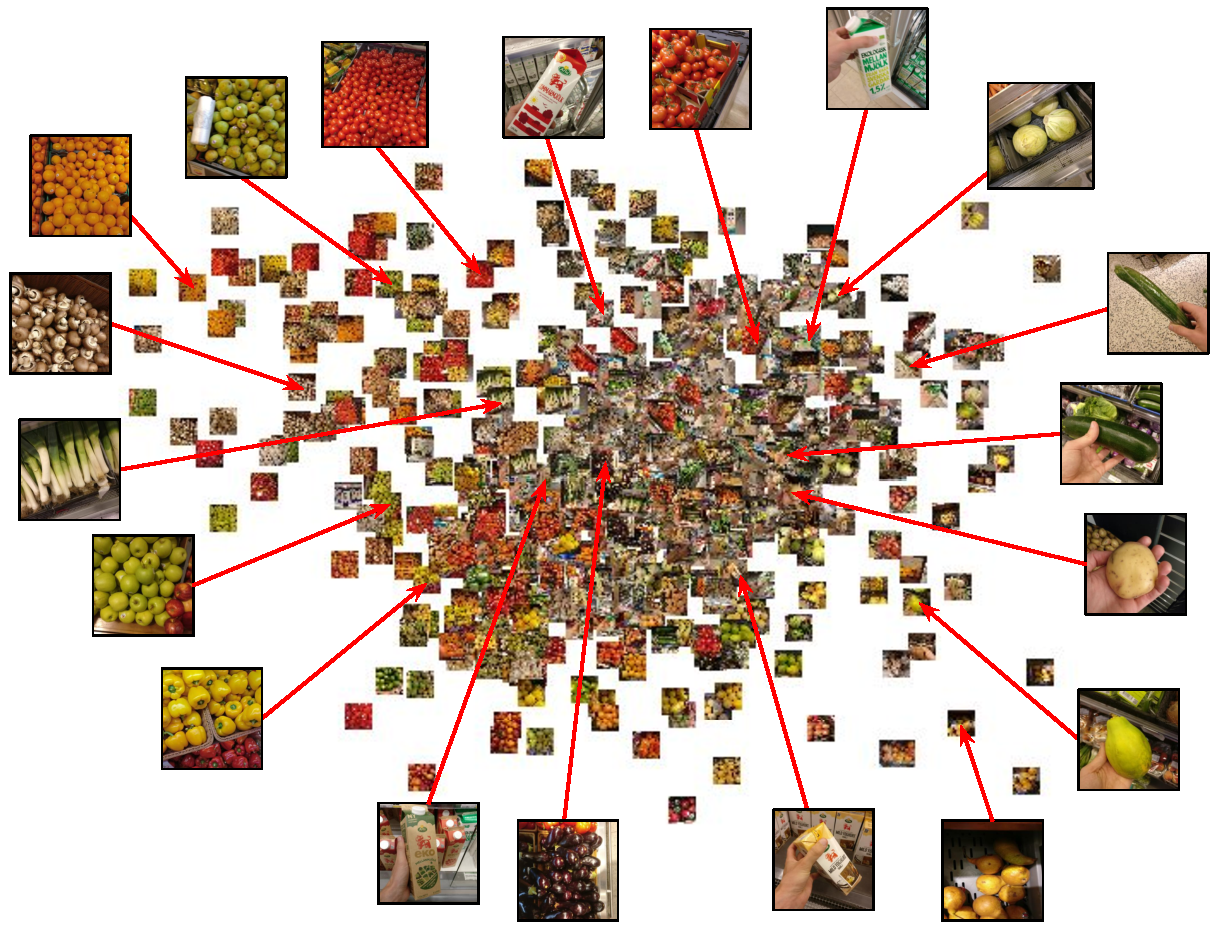
\includegraphics[width=\textwidth]{PaperB/figures_and_tables/private_latent_space_visualizations/vcca_private_ux_space.pdf}
         \caption{$\mu_{x}$ from VCCA-private$_{x w}$}
         \label{fig:pca_vcca_private_xw_ux}
     \end{subfigure} \\
     \begin{subfigure}[b]{0.7\textwidth}
         \centering
         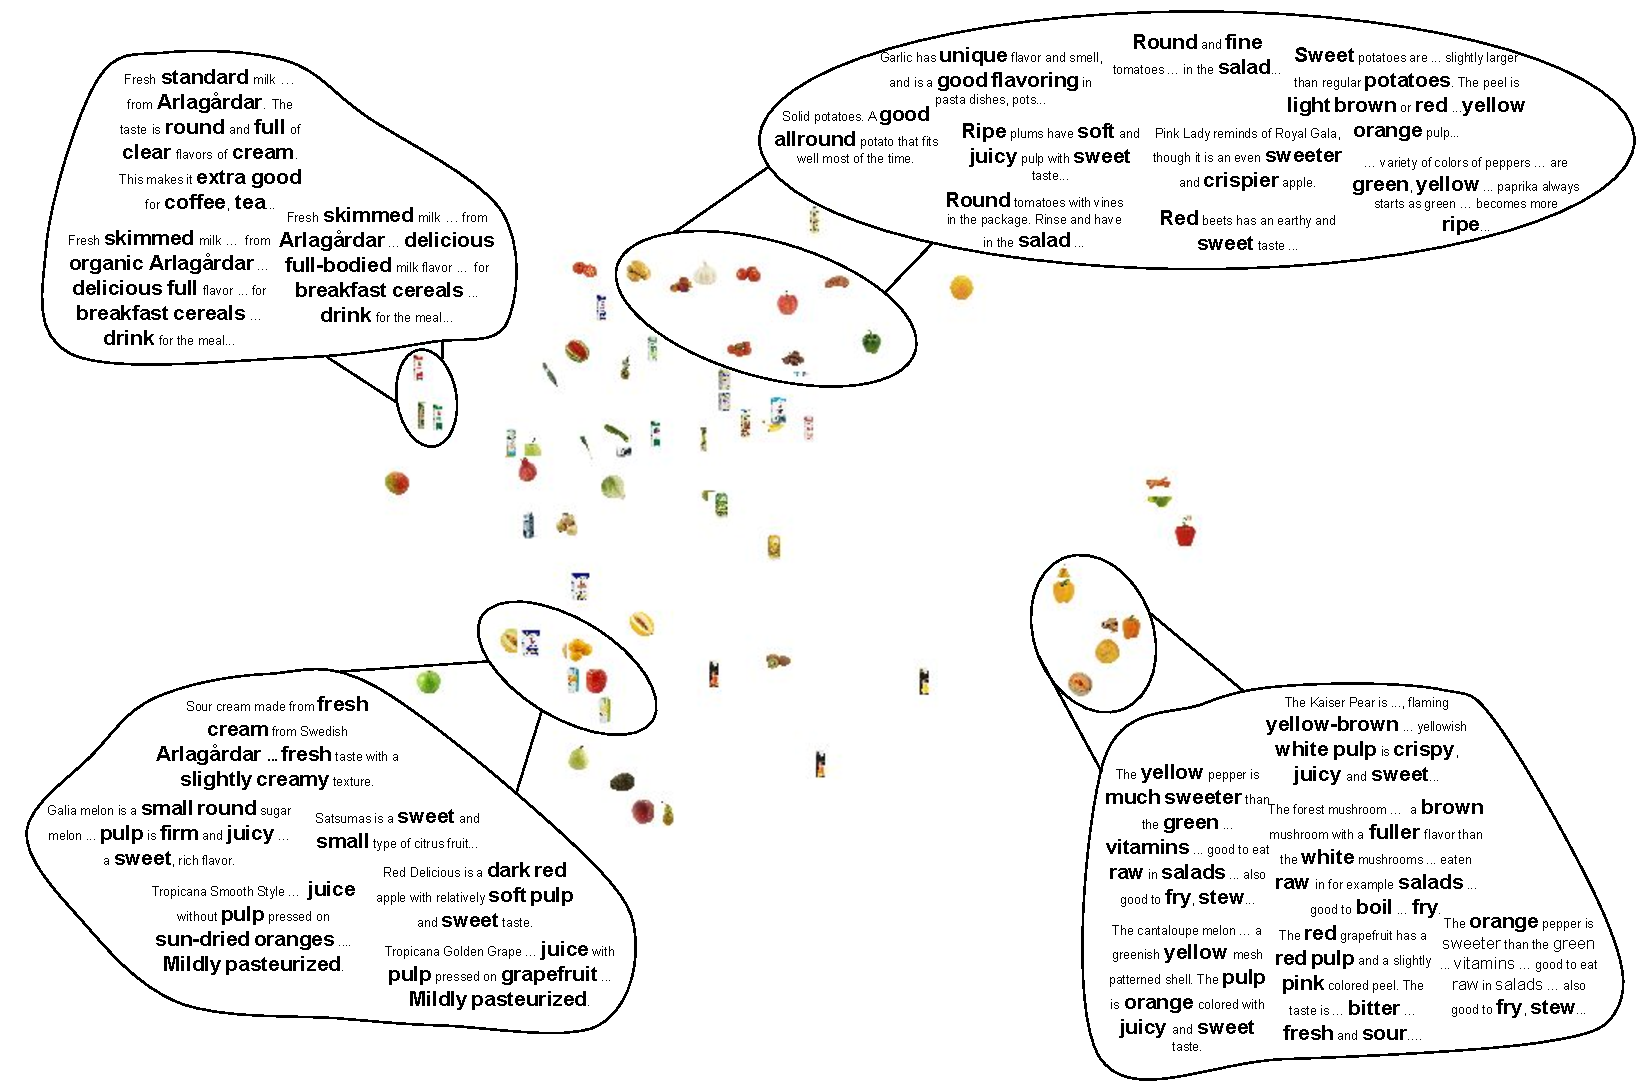
\includegraphics[width=\textwidth]{PaperB/figures_and_tables/private_latent_space_visualizations/vcca_private_uw_space.pdf}
         \caption{$\mu_{w}$ from VCCA-private$_{x w}$}
         \label{fig:pca_vcca_private_xw_uw}
     \end{subfigure} 
    \caption{Visualizations of the latent representations $\mu_{z}$ of a selection of juice packages and yoghurt packages in the Grocery Store dataset. The yellow and green points correspond to the juice and yoghurt packages respectively. The blue points correspond to the other grocery items. 
    	%Abbreviations: VCCA, Variational Canonical Correlation Analysis.
    }
    \label{fig:2d_visualizations_pca_vcca_private_xw}
\end{figure}